\documentclass[11pt,a4paper]{article}
\usepackage[utf8]{inputenc}
\usepackage[italian]{babel}
\usepackage{amsmath}
\usepackage{graphicx}
\usepackage{geometry}
\geometry{a4paper, margin=2.5cm}
\usepackage{float}
\usepackage[hypcap=true]{caption} % Forza i link in alto sopra l'immagine
\usepackage[colorlinks=true, linkcolor=blue, urlcolor=blue]{hyperref} % Deve sempre essere l'ultimo!

\title{Relazione Finale - Modellazione e Simulazioni Numeriche \\ \large Progetto: Transizione di Fase Termodinamica e Algoritmica di Percolazione}
\author{Martin Trajkovski}
\date{\today}

\begin{document}

\maketitle

\section{Introduzione e Obiettivi Analitici}
Questa relazione documenta l'analisi formale del modello base di generazione e frammentazione reticolare noto come "Percolazione 2D" su un assetto a matrice quadrata $L \times L$. Il problema fondamentale non consiste puramente nella validazione visiva della connettività, ma nell'estrarre determinazioni statiche, limiti asintotici e grandezze topologiche che convalidano il quadro teorico delle Transizioni di Fase di tipo termodinamico continuo. L'obiettivo operativo ha previsto il distacco dall'inefficiente algoritmo ricorsivo di \textit{Flood-Fill} avvalendosi dell'architettura \textit{Hoshen-Kopelman} (HK), in modo da abilitare simulazioni \textit{Monte-Carlo} dense ed annullare le penalità di esecuzione computazionale in prossimità della fluttuazione critica.

\section{Ottimizzazione Architetturale: Union-Find e Hoshen-Kopelman}
Il tracciamento dei cluster standard tramite l'immersione ricorsiva o a pila (l'approccio standard \texttt{CercaCluster.m}) presenta un limite strutturale drammatico: valicando la soglia d'aggregazione $p_c \approx 0.60$, il reticolo decanta rapidamente verso un ammasso reticolare unificato. La memoria strutturata subisce un over-saturation costringendo l'algoritmo visivo ad interrogare a ritroso la matrice un quantitativo esponenziale ed irrazionale di volte.

Per superare rigorosamente tale collo di bottiglia, è stata implementata la configurazione \textit{Hoshen-Kopelman (HK)}.
Il codice impiega operativamente i Disjoint-Set (\textit{Union-Find}): il reticolo in input viene esplorato tramite un un'unica scansione cardinale (\textit{Raster Scan}, unicamente asse verticale decrescente ed orizzontale crescente). La predizione assume inferenza sollevando le congiunture sui vicini pre-calcolati (Nord, ovest). L'intuizione logistica prevede non la riscrittura del reticolo fisico ma l'accorpamento virtuale delle etichette (Label) dinamicamente confliggenti dentro uno smistatore virtuale: The \textit{Parent List}. Questo salto prestazionale recide le interrogazioni spaziali ritardate inglobando la valutazione unicamente alla taglia natia dei gridpoint analizzati ($L^2$), determinando una risolvente $\mathcal{O}(N)$.

\begin{figure}[H]
    \centering
    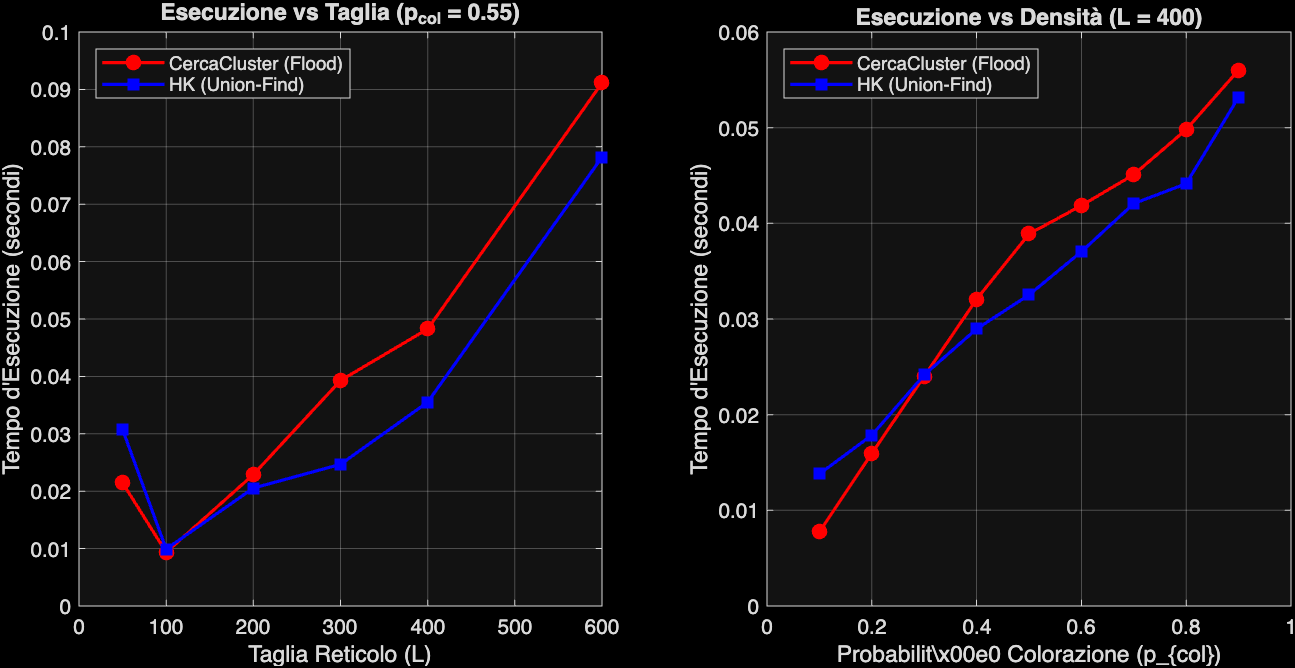
\includegraphics[width=0.9\textwidth]{../Laboratorio_Matlab/Test_efficienza.png}
    \caption{Profilazione dei tempi di esecuzione: comparazione computazionale dell'approccio Flood-Fill contro lo schema Union-Find (HK).}
    \label{fig:efficienza}
\end{figure}

L'evidenza empirica di profilazione in \hyperref[fig:efficienza]{Figura \ref*{fig:efficienza}} palesa il radicale divario algoritmico. Mentre la variante a pila soffre in scalabilità all'allargarsi dei lati dell'arena ($L$) o all'ostruzionismo dettato dall'intensificarsi del riempimento cromatico ($p_{col}$), l'algoritmo Hoshen-Kopelman assorbe invariato l'aumento della massa critica pre-soglia.

\section{Distribuzioni di Connettività, $P_1$ e RACS}
Forte della stabilità computazionale acquisita in ordine temporale per ogni simulazione asparsa, l'analisi vettoriale è stata displicata in altissima densità ($N=200$ invocazioni analitiche) esaminando gli assetti nell'intorno nevralgico della criticità topologica. Ogni serie estrapolata ingloba l'intervallo d'errore del campionamento \textit{Standard Error M.C.}, limitando l'errore apparente a una pura deviazione incerta standard normalizzata.

\begin{figure}[H]
    \centering
    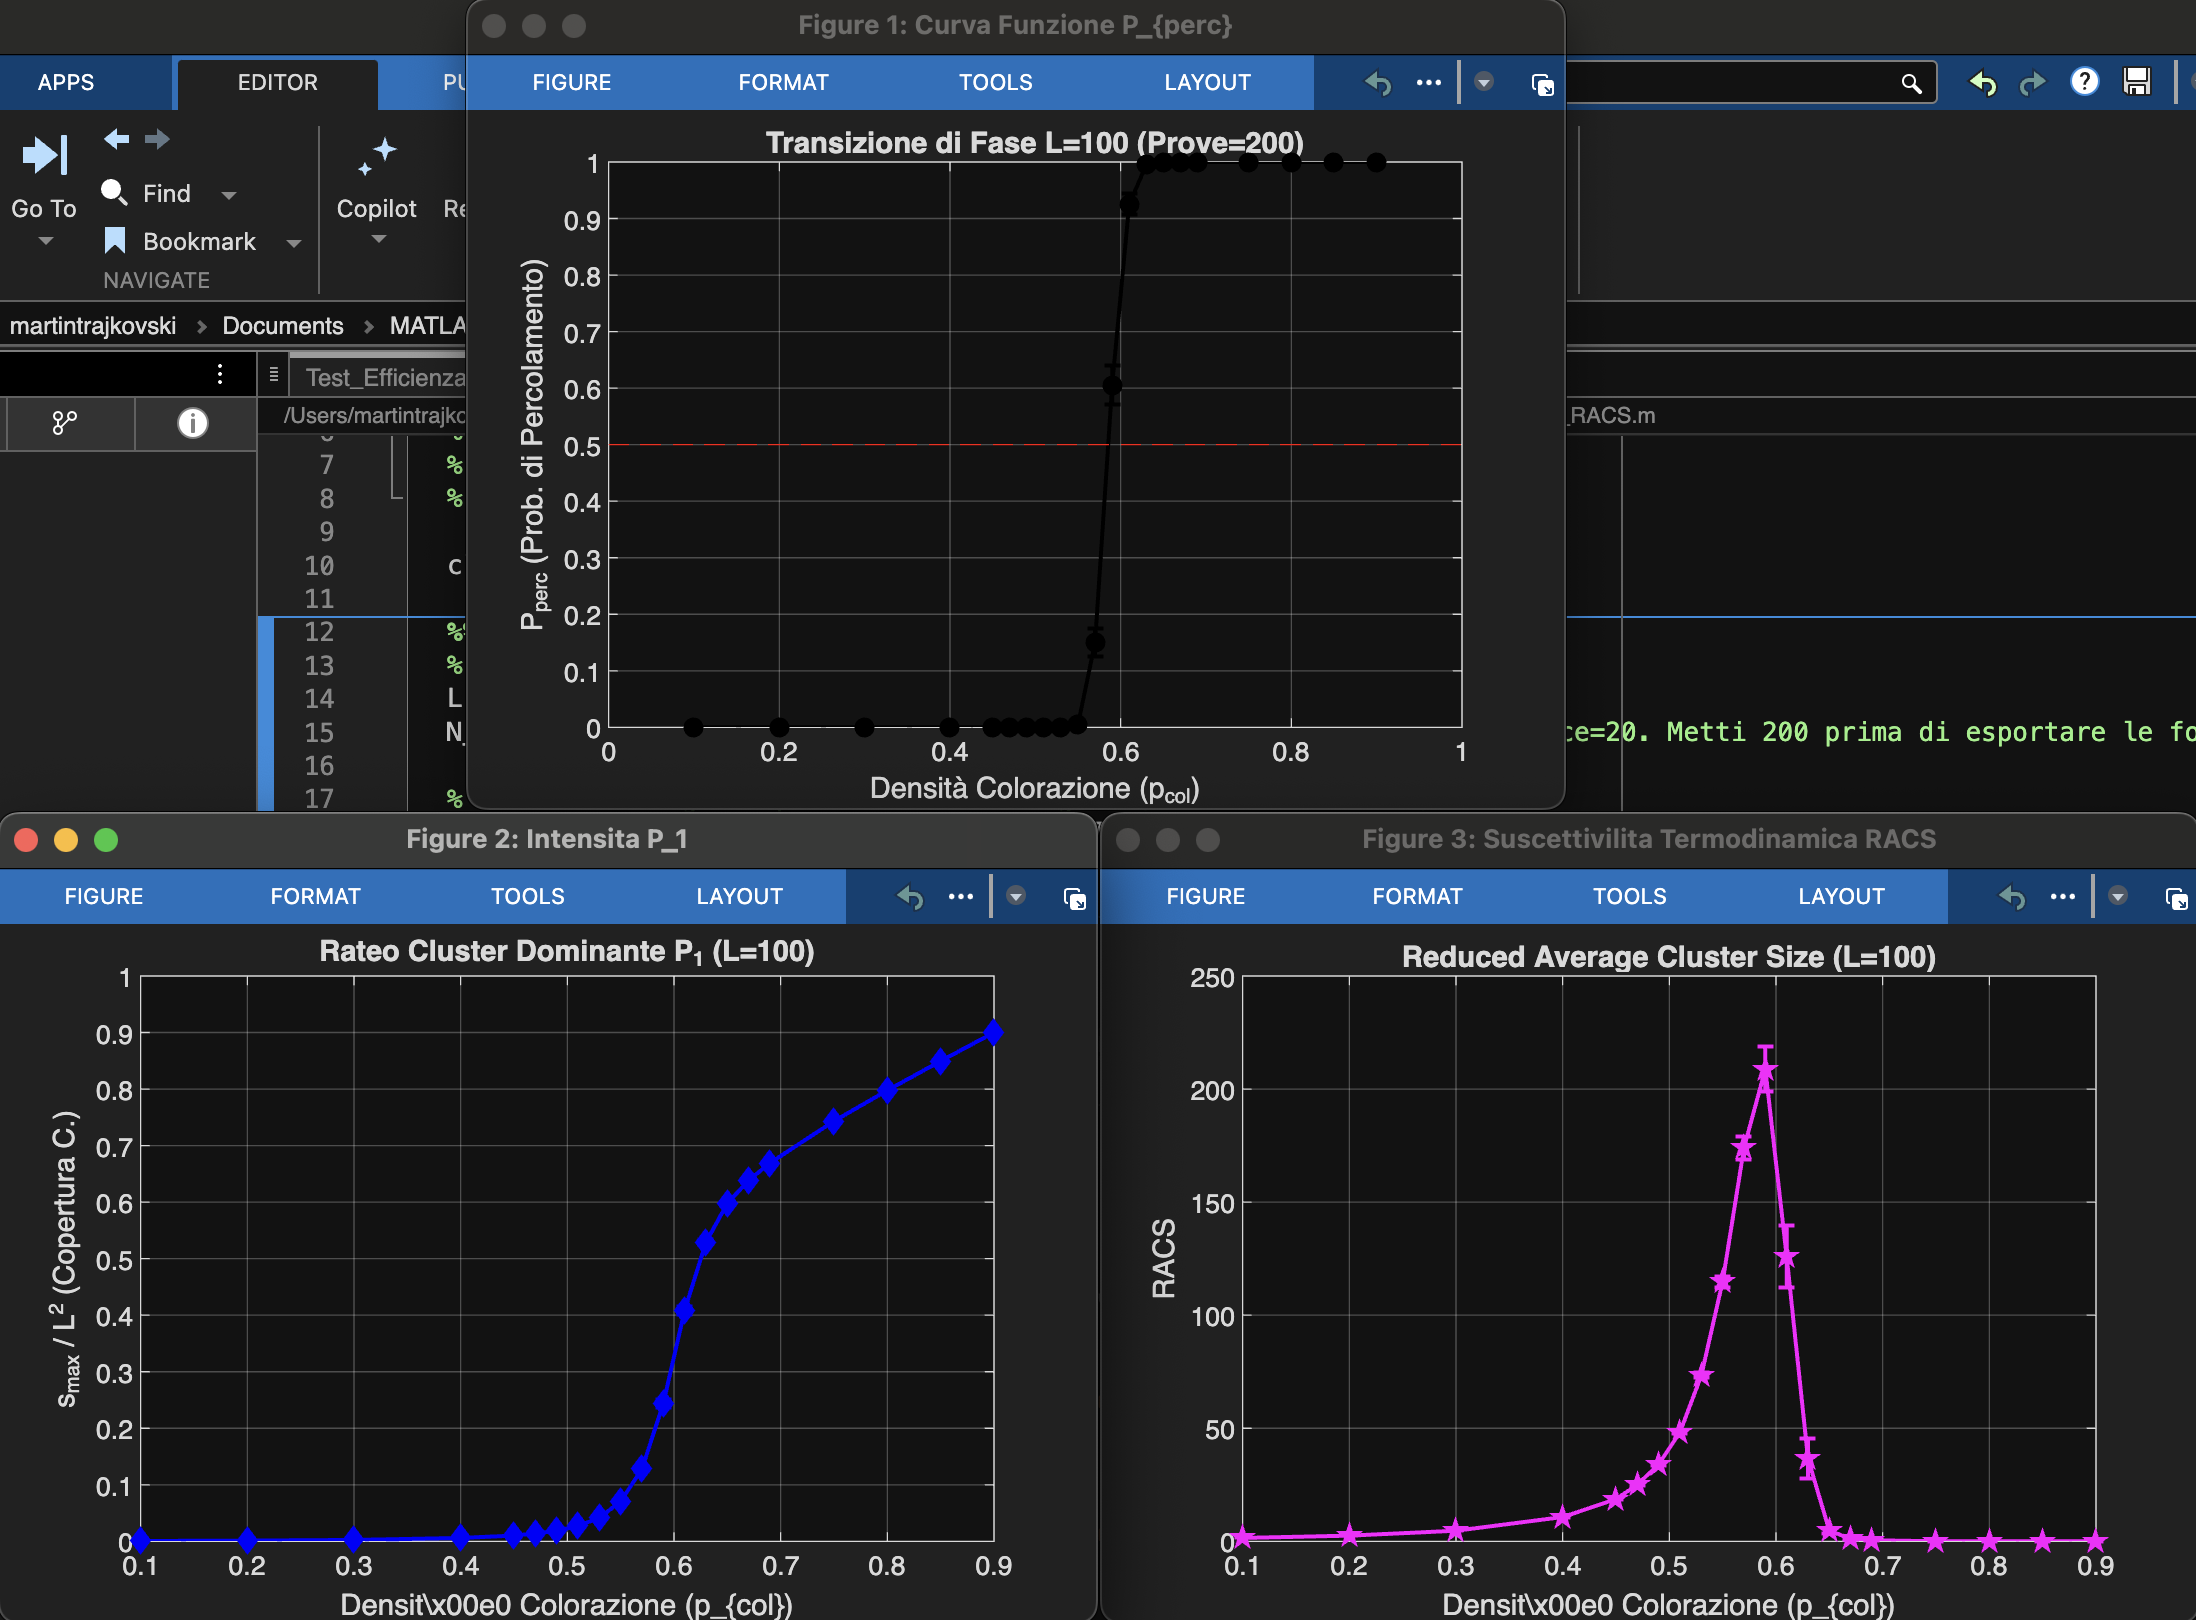
\includegraphics[width=\textwidth]{../Laboratorio_Matlab/analisi_soglia_racs_200.png}
    \caption{Spettro Termodinamico e Soglie: (1) Probabilità di Percolazione Orizzontale/Verticale, (2) Frazione Massica Isolata $P_1$, (3) Media Taglia Cluster Ridotta (RACS).}
    \label{fig:termodinamica}
\end{figure}

L'indagine espone tangibilmente i teoremi asintotici di frontiera (Rif. \hyperref[fig:termodinamica]{Figura \ref*{fig:termodinamica}}):
\begin{itemize}
    \item \textbf{Morfologia a S della Sigmoide (Pannello 1):} Contrariamente al subitaneo e categorico salto del \textit{Gradino di Heaviside} esigibile teoreticamente per reticoli infiniti, il grafico convalida scientificamente l'esistenza empirica di una morfologia smussata "ad S" che regge lo specchio dei test finitamente delineati al calcolatore. Il rateo di penetrabilità delle sponde del reticolo implode e subisce uno sblocco critico superando prepotentemente il margine in bilico posto a $p_{col} \approx 0.59$.
    \item \textbf{Comportamento Organico del Parametro d'Ordine ($P_1$) (Pannello 2):} Palesa l'evoluzione endogena interna all'asseganto dominante: oltrepassata la transizione, cessa l'eterogeneità statistica e la varianza geometrica. Il telaio viene fagocitato interamente dal \textit{Spanning Cluster} che cresce non più in maniera aggregativa sparsa ma ramificandosi quasi a formare l'architettura assiale intera dell'ambiente matematico.
    \item \textbf{Suscettibilità di Transizione RACS (Pannello 3):} La "Radiografia" computazionale prediletta dal modello. Rimuovendo esplicitamente il \textit{Cluster Maggioritario Spanning} dalla funzione (eliminato per decodificare il "rumore" che occulta la transizione), il termine denominatore perde convergenza rispetto al nominatore della massa critica che inizia a deviare esplosivamente originando il fenomeno asintotico noto quale "Vulcano Termodinamico". Tale picco si innesca impercettibilmente a valle del $0.593$, allorché i rimanenti e secondari micro-reticoli lottano disperatamente ingrossandosi prima che l'ulteriore singola molecola accesa finisca per agglutinarli tutti d'un colpo, declassando ed annullando il parametro per l'ingresso nel nuovo equilibrio termodinamico di post-percolazione.
\end{itemize}

\section{Considerazioni Formative in Sede d'Esame}
\subsection*{4.1 Finite-Size Scaling}
Nei modelli in cui un fenomeno esplode in maniera macroscopica si valuta sempre la "Lunghezza di Correlazione Geometrica" ($\xi$). Nell'assunto di cui all'osservazione, l'addolcimento sperimentato attorno ai fianchi della Soglia è strettamente ricondubile "all'Errore Fisico della Memoria di Appoggio". Elementi insiti e raggruppamenti di pixel che in uno spazio di iterazione infinito non dovrebbero neppur lambirsi topologicamente, riescono puramente ed erroneamente (spuntando la percolazione casuale anticipata) a trovare gli angoli laterali costretti dei muri del computer stesso in test per via di $L=100$. Queste limitatezze spiegano con enorme eleganza le derive distorte del reticolo asperso.

\subsection*{4.2 Indipendenza Aleatoria nel Monte Carlo}
Mentre per i test su catena di \textit{Code Infinita (Birth-Death)} vige il vizio di ereditare tempisticamente le saturazioni limitanti, il set di test di Hoshen testé misurato scansa interamente il rumore e l'errore insidioso dell' \textit{Autocorrelazione Temporale}. Ogni esecuzione randomica che compone le medie a base 200 per parametro di Densità, impone una tabula rasa in \texttt{Matlab} in totale distacco da memorie di tracciato pregresso, eludendo i fattori di scarto dell'integrale dei tempi e fornendo purezza accademica alle varianze stampate a video tramite Limite Centrale Universale (CLT).
\end{document}
